\documentclass[9pt,oneside]{amsart}
\usepackage{graphicx}
\usepackage{multicol}
\usepackage{amsmath}
\usepackage{amssymb}
\usepackage[a4paper,width=170mm,top=18mm,bottom=22mm,includeheadfoot]{geometry}
\usepackage{booktabs}
\usepackage{array}
\usepackage{verbatim}
\usepackage{caption}
\usepackage{mathtools}
\usepackage[dvipsnames]{xcolor}
\usepackage{tikz}
\usetikzlibrary{arrows.meta, positioning}
\usepackage{glossaries}
\usepackage{xpatch}
\usepackage[bookmarks=true, unicode=true, pdftitle={RGB I.0: Scalable Consensus for Client-side Validated Smart Contracts}, pdfauthor={Dr. Maxim Orlovsky},pdfkeywords={RGB, Yellow Paper, blockchain, virtual machine, cryptography, decentralised, client-side validation, Bitcoin, Lightning},pdfborder={0 0 0.5 [1 3]}]{hyperref}
%,pagebackref=true

\PassOptionsToPackage{hyphens}{url}\usepackage{hyperref}

\makeatletter
 \newcommand{\linkdest}[1]{\Hy@raisedlink{\hypertarget{#1}{}}}
\makeatother

\usepackage[english]{babel}
\usepackage[autostyle]{csquotes}
\MakeOuterQuote{"}

\usepackage[final]{microtype} % https://tex.stackexchange.com/questions/75140/is-it-possible-to-make-latex-mark-overfull-boxes-in-the-output#comment382776_75142

\DeclareMathAlphabet{\mathpzc}{OT1}{pzc}{m}{it}

\DeclareCaptionFormat{myformat}{#1#2#3\hrulefill}
\captionsetup[figure]{format=myformat}

\makeatletter
\newinsert\copyrightnote@ins
\count\copyrightnote@ins=1000
\dimen\copyrightnote@ins=8in
\newcommand*\copyrightnote@hook
  {%
    % place 
    \unvbox\copyrightnote@ins
    \global\let\@makecol\copyrightnote@makecol
  }
\let\copyrightnote@AtBeginDocument\AtBeginDocument
\AtBeginDocument{\let\copyrightnote@AtBeginDocument\@firstofone}
\newcommand*\copyrightnote@firstuse
  {%
    \gdef\copyrightnote@firstuse
      {\global\skip\copyrightnote@ins=\bigskipamount\gdef\copyrightnote@firstuse{}}%
    % backup to later restore it
    \global\let\copyrightnote@makecol\@makecol
    % after the actual footnotes are placed we place something else
    \xpatchcmd\@makecol{\unvbox\footins}{\unvbox\footins\copyrightnote@hook}
      {}{\GenericError{}{patching @makecol failed}{}{}}
    \copyrightnote@AtBeginDocument
      {%
        % trick the output routine to think there are footnotes, even if there
        % are none
        \ifvoid\footins
          \insert\footins{}% 
        \else
          \global\skip\copyrightnote@ins=\bigskipamount
        \fi
      }%
  }
\newcommand\copyrightnote[1]
  {%
    \copyrightnote@firstuse
    \copyrightnote@AtBeginDocument
      {%
        \insert\copyrightnote@ins
          {%
            \reset@font\footnotesize
            \interlinepenalty\interfootnotelinepenalty
            \splittopskip\footnotesep
            \splitmaxdepth\dp\strutbox
            \floatingpenalty\@MM
            \hsize\columnwidth
            \@parboxrestore
            \color@begingroup
            \parindent1em
            \noindent
            \hskip1.8em
            \ignorespaces #1\@finalstrut\strutbox
            \color@endgroup
          }%
      }%
  }
\makeatother

\def\bitcoin{%
  \leavevmode
  \vtop{\offinterlineskip %\bfseries
    \setbox0=\hbox{B}%
    \setbox2=\hbox to\wd0{\hfil\hskip-.03em
    \vrule height .3ex width .15ex\hskip .08em
    \vrule height .3ex width .15ex\hfil}
    \vbox{\copy2\box0}\box2}}

\newenvironment{coltable}
  {\par\bigskip\noindent\minipage{\columnwidth}\centering}
  {\endminipage\par\bigskip}

\makeglossaries
\loadglsentries{glossaries}
\renewcommand*{\glstextformat}[1]{\textit{#1}}

\title[RGB I.0: Scalable consensus for client-side validated smart contracts]{RGB I.0\\Scalable consensus for client-side validated smart contracts\\ \it \today}
\author[M. Orlovsky]{Dr. Maxim Orlovsky}
\dedicatory{Institute for Distributed and Cognitive Systems, LNP/BP Labs \& UBIDECO Labs, Lugano, Switzerland; \\
Pandora Prime SA, Neuchatel, Switzerland}

\copyrightnote{Copyright: \copyright 2025 RGB Consortium, \copyright 2019-2025 Dr. Maxim Orlovsky. All rights reserved.}
\copyrightnote{License: Creative Commons BY (CC-BY)}

\begin{document}
\pagecolor{yellow!10}

\begin{abstract}
The paper defines a novel type of consensus for a distributed smart contract system,
named RGB, which is based on the concept of client-side validation,
separating the contract state and operations from the blockchain.
With this approach, contracts are sharded (each contract is a standalone shard),
kept, and validated only by contract participants,
providing native scalability and privacy mechanisms,
exceeding all existing blockchain-based smart contract systems
while not compromising on security or decentralization.
The system is designed to operate on top of compatible layers 1,
such as an UTXO-based blockchain (e.g., Bitcoin)
without relying on it for transaction ordering or state replication.
Instead, RGB keeps the state client-side,
operating as partially replicated state machines (PRiSM).
It employs a novel SONIC (State machine with Ownership Notation Involving Capabilities)
architecture, which provides capability-based access control to the contract state,
individually owned and operated by a well-defined contract parties
via novel single-use seal mechanism.
RGB does state validation using zk-AluVM virtual machine,
designed to support zk-STARK provers.
It has a single security assumption of the collision-resistance hash function
and, thus, is quantum-secure.
The proposed RGB consensus is distinct from traditional
blockchain-based smart contract systems;
it is scalable, provably-secure, and formally verifiable.
\end{abstract}

\maketitle

\thispagestyle{empty}
\setlength{\columnsep}{20pt}
\begin{multicols}{2}

\section{Introduction}

\subsection{Background}

The idea of smart contracts, originating from Nick Szabo \cite{Szabo},
has been an inspiration for almost a generation of researchers and innovators.
Nevertheless all existing attempts for building permissionless smart contracts
were based on fully-replicable blockchain consensus,
and thus were failing to solve the trilemma of being
\begin{itemize}
    \item scalable as $O(1)$, or at least as $O(\log n)$;
    \item universal (``Turing-complete'');
    \item decentralized, permissionless, and trustless.
\end{itemize}

The main reason was the fact that all the mentioned approaches require
all participants to verify the state and state transition function of all world smart contracts,
which, for obvious reasons, cannot scale.

Multiple attempts has being made to solve blockchain non-scalability issue
via adding layers on top: sidechains \cite{sidechains, drivechains},
statechains \cite{statechains}, state channels \cite{lightning, eltoo}, plasma \cite{plasma},
optimistic rollups \cite{optimism}, validiums \cite{validium},
zk-rollups \cite{zk-rollups, Cairo, mina}.
However, all of the approaches result in either
centralization, higher trust assumptions, possibility of a censorship,
or suffer from economical non-scalability \cite{drivechainsucks, plasmasucks, rollupsucks},
like in the case of the infamous Lightning network inbound liquidity \cite{lightningsucks1, lightningsucks4},
routing \cite{lightningsucks2} and centralization issues \cite{lightningsucks3, lightningsucks5}.
Also, all layer 2 solutions has the state which must be eventually published
to the blockchain, so, the state transition business logic also has to be global.
This becomes especially an issue for blockchains designed for a
``Turing-complete'' contracts, serving a complete VM,
like in Ethereum \cite{ethereum} or Cardano \cite{cardano}.
Thus, all of them may save only a constant factor and cannot solve the fundamental
limitation created by a blockchain-based consensus.

\subsection{Client-side Validation}

This problem can be addressed with \emph{client-side validation} –
the paradigm proposed by Peter Todd in 2016 \cite{CSV}.
Its core idea is that state validation in a distributed system
does not need to be performed globally by all parties of a decentralized protocol;
instead, only parties involved in (or affected by)
a specific state transition need to perform the validation.
With this approach it is sufficient to publish only a cryptographic commitment,
with no state data, and the parties of the specific transaction
be able to verify that it is correct, final and singular —
without the rest of the world even knowing of it.
This is achievable with a new class of cryptographic protocols,
also proposed by Peter Todd, named single-use seals \cite{SUS1, SUS2, SUS3, SUS4},
which allow proving both finality and singularity\footnotemark
of a state transition in a noninteractive way.

\footnotetext{By \emph{singularity} here we mean a property that any
atom of a contract state can be updated once and only once, in a non-concurrent way.
In case of an UTXO model used in Bitcoin-type blockchains \cite{UTXO}
this is also named an \emph{anti-doublespending} property,
but in more generic context of UTXO-based smart contracts we use the term
\emph{singularity} of state updates.
\vspace{6pt}
\hrule}

Based on the ideas of Peter Todd, Giacomo Zucco had proposed
an early idea of RGB as a client-side validated asset system,
leveraging Bitcoin transactions (both on-chain and off-chain, like in Lightning network)
for the \emph{single-use seals} protocol \cite{Zucco}.
However, this early idea and prototype implementation was lacking programmability,
support for non-trivial state, ability for a Bitcoin UTXO to be used by multiple assets,
and was not zk-friendly.

\subsection{Our Contribution}

In our work, we have developed the original idea of RGB into the first universal
client-side validated distributed smart contracting system,
solving all the above-mentioned issues.
RGB employs a novel SONIC (State machine with Ownership Notation Involving Capabilities) architecture,
leveraging zk-AluVM virtual machine \cite{AluVM} and zk-STARKs \cite{zkSTARKs}
for scalability, security, and formal verification.
The protocol operates as partially replicated state machines (PRiSM);
it uses polynomial computation and capability-based access control,
which makes it distinct from traditional smart contract systems.
The protocol operates on top of a UTXO-based blockchain~\cite{UTXO}
(so-called \gls{layer~1}) using it as a finality gadget;
however, the blockchain consensus is not used for ordering of transactions or storing a state,
unlike in all other smart contract systems.
Thus, \gls{layer~1}, in strict computer science terms,
does not serve as an RGB consensus by itself,
since it does not fulfill any of the properties defining
a distributing consensus protocol \cite{consensus}:
\noindent\nopagebreak
\begin{itemize}
    \item ordering of transactions (RGB transactions are not published or broadcast via blockchain);
    \item state machine replication (no state is replicated via \gls{layer~1});
    \item atomic broadcasts (since the ordering of \gls{layer~1} transactions does not matter for RGB).
\end{itemize}

Instead, RGB runs its own \emph{client-side validated consensus},
where blockchain consensus acts as one of the components:
the \emph{single-use seal} medium, or \gls{layer~1} \cite{LNPBP8}.
The consensus is quantum-secure (as long as the underlying layer~1 network is quantum-secure),
being based on cryptographic hash functions and not using any elliptic-curve cryptography.
The consensus does not rely on any security assumptions other
than the collision resistance of the selected cryptographic hash function.

This paper provides a complete formal description of the first version of the RGB consensus
released to the production, named \textbf{RGB I.0}.

\section{Used Notations}

We use standard mathematical notation, including operators of set theory.

\subsection{Data types}

Data types are defined using standard sets, such as
natural numbers $\mathbb{N}$, integers $\mathbb{Z}$,
nonzero natural numbers $\mathbb{N}^+ \triangleq \mathbb{N}\setminus\{0\}$
and finite field $\mathbb{F}_q$ (where $q$ is the order of the finite field).
The bit dimensions (except for the finite field elements) are given as a subscript,
like $\mathbb{N}_{256}$, with $\mathbb{N}_8$ used for both 8-bit unsigned integers and bytes.

Binary strings (scalar arrays) of fixed size are given using power notation,
for instance, $\mathbb{N}_8^{32}$ is a 32-byte string\footnote{
The difference between $\mathbb{N}_8^{32}$ and $\mathbb{N}_{256}$ lies in the fact that
the former is a byte string with a fixed encoding,
while the latter is a natural number, which may be serialized either
little-endian or a big-endian.
For little-endian serialization $\mathbb{N}_{256}|_\mathsf{littleEndian} \equiv \mathbb{N}_8^{32}$.
RGB consensus uses only little-endian serialization,
and thus the two representations are equivalent}.

Named data types are represented with capital Latin letters using \LaTeX\ $\mathbb{MATHBB}$ font style.
For example, the Boolean type is defined as a set $\mathbb{B} \triangleq \{0, 1\}$.

Scalar variables are given with Latin and Greek lowercase letters.
The basis for nondecimal scalar literals is given in subscript,
for example, $10_2$ equals $2$ in decimal notation. Decimal literals omit the basis subscript.

\subsubsection{Product types}

Tuples (ordered fixed-size set of objects of different types)
are shown with angular brackets $\langle \ldots \rangle$,
which contains a list of the tuple fields.

Immutable tuple fields are specified with small Latin serif letters
(such as $\mathsf{a}, \mathsf{x}$) or capital Greek letters ($\Theta$).

Mutable tuples that may change over time (tuple variables) are denoted
with capital Latin serif letters (like $\mathsf{C}$). To represent
a sequence or individual tuple values which evolve over time (like state objects),
with individual values being a lowercase indexed version of the same letter
($\mathsf{c}_0, \mathsf{c}_i$, etc.)

Tuple fields may be named or unnamed.
To represent a named field of a tuple we use subscription made with serif font,
such as in $\mathsf{c}_i \triangleq \langle \mathsf{C_{Id}}, \ \ldots \rangle$.

\subsubsection{Sum types}

Enums (sum types) are represented as sets, and enum variables as values
picked from a set of allowed values.
Optional values thus belong to the set $\{ \varnothing, x \}$.

Enums with no associated data are tagged with names,
and a $\mathbb{N}_8$ value used in data serialization, is given as a subscript;
for example $\{ \mathsf{false}|_{=0}, \mathsf{true}|_{=1} \}$.

Enum values with associated data display variants or literals as variables of the corresponding type;
they can include tagged names as a part of the subscript: $\{ x|_{\mathsf{variantA}=0}, y|_{=1} \}$.

\subsubsection{Collections}

Collections (variable-size sets of objects of the same type, ordered or unordered)
are denoted with Latin uppercase calligraphic letters (like $\mathcal{S}$).
For representing set elements, we use braces $\{\ldots\}$ and the set builder notation \cite{setbuilder}.
Ordered collections are indexed with subscripts: $s_i \in \mathcal{S}$.

The type of variable-sized sets is given as an element type with a power component
specifying the range of cardinality allowed for the set.
For example, $\mathbb{N}_8^{[0, 2^{32})}$ indicates a sequence of bytes with cardinality (length)
in the range of $0$ to $2^{32} - 1$.

Set definitions use a subscript to specify the ordering:
$\{ \cdots \}_\prec$ for partially ordered sets;
$\{ \cdots \}_\preceq$ for totally ordered sets;
no index for unordered sets.

UTF-8 Unicode strings are represented as a sequence made up of $\mathbb{U}$ set elements;
ASCII strings as a sequence made up of $\mathbb{S}$ set elements.
If there are constraints on the type of ASCII characters that can be used in a string,
the constraint is either given verbally as an index (for example, $\mathbb{S}_\mathsf{printable}$),
or as a wildcard $\mathbb{S}_*$ with detailed explanation of the constraints given in the text.

Maps are written as a surjective function, mapping each element of a set of keys to a value:
$M: \{ \forall k \in \mathcal{K} \rightarrow v \}$.
The size of the key set may be specified as a power:
$M: \{ \forall k \in \mathcal{K} \rightarrow v \}^{[0, 10)}$.

\subsection{Function types}

Functions with a well-defined algorithm are denoted by small-case Latin serif names,
followed by a colon, function domain, arrow, and function codomain,
such as $\mathsf{evaluate}: \mathcal{A} \rightarrow \mathcal{B}$.
The application of the function to the arguments is written as $\mathsf{evaluate}(a_i)$.
Variables having function type are written as small Greek letters in italics, $\phi$,
and their application as $\phi(x)$.
Functions depending on their previous values are defined using
$\mapsto$.

\subsection{Operators}
The order of the elements in a set is indicated by $\succ$ and $\prec$.
New terms are defined by $\triangleq$.

Bitwise binary operations are specified with $\&$ (AND), $|$ (OR),
$\nleftrightarrow$ (XOR) and $\thicksim$ (NOT)

Logical conditions are specified with $\land$ (AND), $\lor$ (OR) and $\lnot$ (NOT).
Operator $\stackrel{?}{=}$ performs equivalence test and results in a Boolean value.

Operator $\Longleftrightarrow$~is used for \emph{if and only if} condition,
$\Rightarrow$~for \emph{than}, $\nRightarrow$~for \emph{else}, $\perp$~for program termination.

\section{Protocol Overview}

In technical terms, RGB operates as \emph{partially replicated state machines} (PRiSM),
which uses \emph{polynomial computer architecture} SONIC
(State machine with Ownership Notation Involving Capabilities).

\emph{Partially replicated} means that the state is not replicated
as a whole in all instances of the state machine;
instead, only a part of the state required by each of the instances is propagated.

\emph{Polynomial computer} means that the trace of the operations can be arithmetized to polynomials,
making it possible to use any zk-STARK prover for zero-knowledge compression.

\emph{Ownership notation involving capabilities} means that some types of state in RGB
are assigned to specific parties (actors), and this assignment is made using \emph{capabilities},
which are implemented using a single-use seal cryptographic scheme.

The principal components of the RGB consensus design are the following:
\begin{itemize}
  \item SONIC polynomial computer (its consensus-related layer named ``UltraSONIC'')
  with capability-based memory and zk-AluVM virtual machine
  used for contract state evaluation/validation;
  \item RGB contracts with their state, operations and state transitions;
  \item single-use seals, for providing capabilities,
  control of state transition singularity and the finality;
  \item commitment schemes, using cryptographic hash functions.
\end{itemize}

The version of RGB consensus described in this document is named \textbf{RGB-I.0}.
You can find more about RGB version numbering in the RGB-6 standard \cite{RGB6}.

\section{SONIC Architecture}\label{Sonic}

Most of the modern computers use von Neumann \cite{vonNeumann},
Harvard, and modified Harvard architecture \cite{Harvard}.
While offering a convenient user experience, these architectures were not designed neither for
arithmetization, required in creation of zk-STARK proofs, nor for distributed systems,
nor for security and formal verification.
For example, random-memory access has been the source
of most hacks and security breaches for more than 50 years \cite{RAMsucks1, RAMsucks2, RAMsucks3}.

Although it is possible to adopt von Neumann-style or Harvard architecture
with RAM for zk-STARK provers (one may refer to Cairo \cite{Cairo}),
this results in large proof size,
high computational resource demand for producing zk-proofs,
and no guaranteed ability to perform termination and
other forms of formal analysis of an arbitrary program.
Instead of following such an approach, RGB is using a different architecture,
named SONIC (see Figure \ref{fig:arch}),
which is specifically designed for formal verification, UTXO-based models, and security.

\end{multicols}
\begin{figure}[h]
    \caption{Comparison of different computer architectures}
    \label{fig:arch}

    \centering
    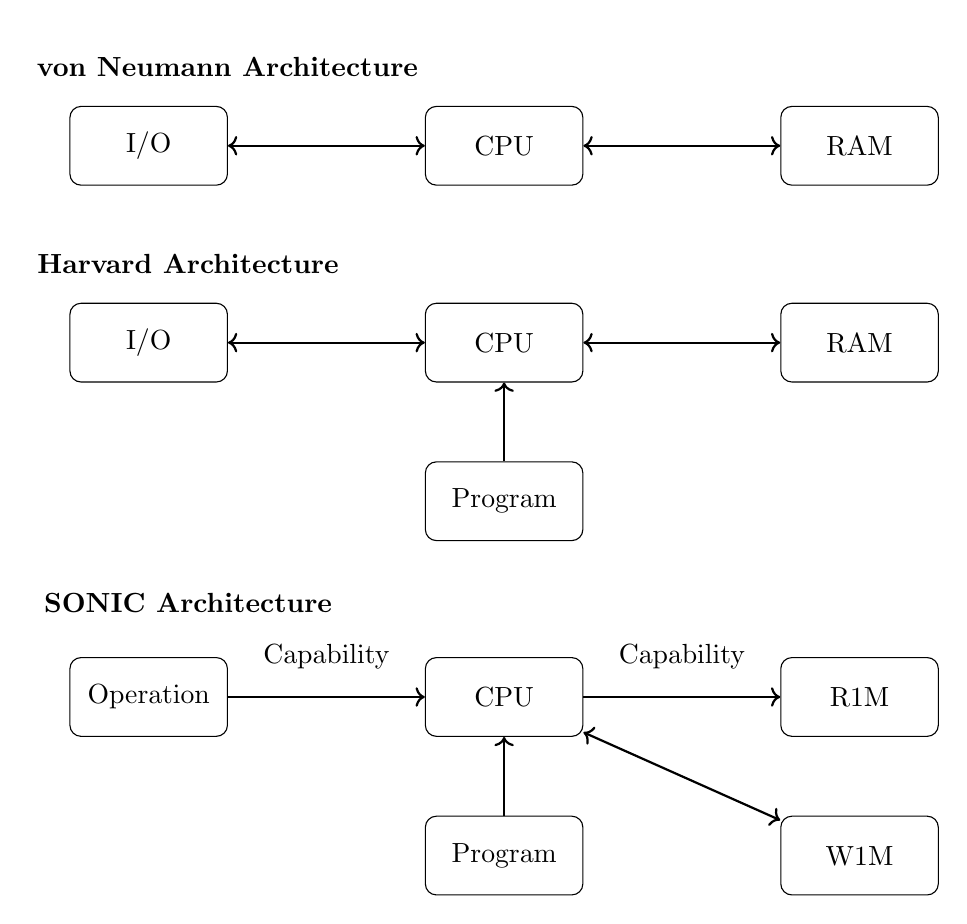
\begin{tikzpicture}[
        node distance=1cm and 2.5cm,
        every node/.style={draw, rounded corners, minimum width=2cm, minimum height=1cm, align=center},
        capability/.style={->, thick},
        dataflow/.style={<->, thick},
        flow/.style={->, thick}
    ]
    
    % von Neumann Architecture
    \node[draw=none, align=left] at (-5,3) {\textbf{von Neumann Architecture}};
    \node (IO1) at (-6,2) {I/O};
    \node (CPU1) [right=of IO1] {CPU};
    \node (RAM1) [right=of CPU1] {RAM};
    
    \draw[dataflow] (IO1) -- (CPU1);
    \draw[dataflow] (CPU1) -- (RAM1);
    
    % Harvard Architecture
    \node[draw=none, align=left] at (-5.5,0.5) {\textbf{Harvard Architecture}};
    \node (IO2) at (-6,-0.5) {I/O};
    \node (CPU2) [right=of IO2] {CPU};
    \node (RAM2) [right=of CPU2] {RAM};
    \node (Program1) [below=of CPU2] {Program};
    
    \draw[dataflow] (IO2) -- (CPU2);
    \draw[dataflow] (CPU2) -- (RAM2);
    \draw[flow] (Program1) -- (CPU2);
    
    % SONIC Architecture
    \node[draw=none, align=left] at (-5.5,-3.8) {\textbf{SONIC Architecture}};
    \node (Operation) at (-6, -5) {Operation};
    \node (CPU3) [right=of Operation] {CPU};
    \node (R1M) [right=of CPU3] {R1M};
    \node (W1M) [below=of R1M] {W1M};
    \node (Program2) [below=of CPU3] {Program};
    
    \draw[capability] (CPU3) -- (R1M) node[midway, above, draw=none] {Capability};
    \draw[capability] (Operation) -- (CPU3) node[midway, above, draw=none] {Capability};
    \draw[dataflow] (CPU3) -- (W1M);
    \draw[flow] (Program2) -- (CPU3);
    
    \end{tikzpicture}
\end{figure}
\begin{multicols}{2}

The architecture uses zk-AluVM virtual machine, immutable memory cells of two types
(read-once memory, R1M; and write-once memory, W1M), and capability-based R1M access.

\subsection{zk-AluVM virtual CPU}\label{AluVM}

zk-AluVM is a pure functional RISC virtual machine
designed for deterministic portable computing tasks \cite{zkAluVM}.
It is built using AluVM (``algorithmic logic unit VM'') \cite{AluVM, AluVMCrate},
a modular framework for creating RISC instruction set architectures (ISA)
and registry-based virtual machines, based on category theory.

\subsubsection{Instruction Set Architecture}

zk-AluVM extends the AluVM execution control flow ISA (see Table \ref{tab:aluvm})
with \textbf{GFA256} ISA for arithmetic operations
with finite field elements (see Table \ref{tab:gfa256}).
It is further extended by \textbf{USONIC} ISA
for accessing operation data and memory (see Table \ref{tab:usonic}).
The complete specification on the instruction set architecture is given in Appendix \ref{ap:ISA}.

\subsubsection{Control Registers}\label{Registers}

The control registers are part of the base AluVM ISA.
They are used for the program execution workflow and do not participate
as explicit arguments for the instructions; however, their value may be accessed or changed
by some of the instructions, as specified in Appendix \ref{ap:ISA}.

\begin{description}
\item[CK] Check register with values taken from $\{\mathsf{ok}|_{=0}, \mathsf{failire}|_{=1}\}$.
    On a failure (like accessing register in \texttt{None} state, zero division, etc.)
    the register is set to the failed state.
    Can be reset if \textbf{CH} is \texttt{false}.
\item[CH] Halting register holding a Boolean value.
    Indicates whether a program must halt the moment \textbf{CK}
    is set to the failed state for the first time.
\item[CO] Test register, which acts as a Boolean test result.
    Its value is checked by branching and some halting instructions.
\item[CA] Complexity accumulator / counter, a $\mathbb{N}_{64}$ number.
    Each instruction has a \emph{computational complexity measure}.
    This register sums up the complexity of the instructions executed.
\item[CL] Complexity limit, as an optional value $\{\varnothing, \mathbb{N}_{64}\}$.
    If the register has a value, once \textbf{CA} reaches or exceeds it,
    the VM will set \textbf{CK} to the failed state.
\item[CS] Call stack, $\{ \mathbb{E} \}^{[0, 256)}$, listing call entry points
    (see the definition of the entry point in Section \ref{Program} and equation \ref{eq:e}).
\end{description}

\subsubsection{\textbf{GFA256} Registers}

The \textbf{GFA256} ISA defines \textbf{FQ} constant (read-only) register,
which contains the order $q$ of the used finite field $\mathbb{F}_q$; and
16 general registers to store finite field element values,
from \textbf{E1} to \textbf{E8}, and from \textbf{EA} to \textbf{EH}.
All registers are equivalent in their functionality and can be used
as arguments in the instructions shown in Table \ref{tab:gfa256}.

\subsubsection{\textbf{USONIC} Registers}

The \textbf{USONIC} ISA extension defines four $\mathbb{N}_{16}$ registers,
\textbf{UI1-UI4}, which acts as operation input and output iterators.
They are initialized with zero, and increment on each data load instruction,
such that destructible and immutable operation inputs and outputs may be
iterated one after another.

For the details on how individual operations work with these registers
please refer to the table \ref{tab:usonic}.

\subsection{Memory}\label{Memory}

The SONIC architecture supports two types of addressed memory:
\begin{description}
\item[Read-once memory] (R1M), or \gls{destructible memory} $\mathcal{D}$,
    having capability-based access and used for storing \gls{owned state}
    accessible only by a valid actor providing a 256-bit \gls{authentication token};

\item[Write-once memory] (W1M), or \gls{immutable memory} $\mathcal{I}$,
    which can be accessed by any party and is used to define a \emph{global contract state}.
\end{description}

Both types of memory are made of addressable memory cells.
An address consists of a 256-bit id of an operation and 16-bit output number
which creates the memory cell:
\noindent
\begin{gather}
\mathbb{A} \triangleq \mathbb{N}^{32}_8 \times \mathbb{N}_{16} \\
\mathsf{r} \triangleq \langle \mathsf{Id}(c_i), j \rangle \in \mathbb{A}
\end{gather}

Memory data are based on \gls{composed value} data type,
which is an ordered sequence from zero to four finite field elements:
\noindent
\begin{equation}
\mathbb{V} \triangleq \bigcup_{n=0}^{4} \mathbb{F}_q^n
\end{equation}

\subsubsection{R1M Memory}\label{R1M}

\Gls{read-once memory} cell consists of a single \gls{composed value} $\sigma$,
an \gls{authentication token} $\alpha$, and an optional \gls{locking condition} $\mathcal{L}$:
\noindent
\begin{gather}
\mathbb{D} \triangleq \mathbb{V} \times \mathbb{F}_q \times \{ \varnothing, \langle \mathbb{V}, \{ \varnothing, \mathbb{E} \} \rangle \} \\
\forall \mathsf{d}_i \in \mathcal{D}(\mathsf{a}) : \mathsf{d}_i \triangleq \langle \sigma, \alpha, \mathcal{L} \rangle \in \mathbb{D}
\end{gather}

A locking condition, when present as $\langle \Theta, \ell \rangle \in \mathcal{L} \setminus \{ \varnothing \}$,
consists of an auxiliary data $\Theta$ and an optional entry point $\ell \in \mathbb{E}$ to a verification program
(for the definition of $\mathbb{E}$ please refer to (\ref{eq:e})).

The locking script, when present as $\varepsilon \in \ell \setminus \{ \varnothing \}$,
is an entry point into the AluVM program (see next section),
which should succeed on execution in order for the cell to be read and destroyed.

The auxiliary data $\Theta$ may be used by a codex verifier script or the custom locking script $\varepsilon$
to check the satisfaction of the lock conditions with an input-specific witness $\Omega$,
which will come from the spending operation input (see Section \ref{Input}).
For example, $\Theta$ may be a value of a public key,
and the \gls{input-specific witness} $\Omega$ will have a signature,
while the script $\varepsilon$ will validate the signature for that key.

Destructible memory cells are destroyed on the first read and cannot be accessed or referenced anymore.

\subsubsection{W1M Memory}\label{W1M}

\Gls{immutable memory} cells consist of a single \gls{composed value} $\varsigma$,
and an optional binary raw data $\mathcal{R}$, up to $2^{16}$ bytes:
\noindent
\begin{gather}
\mathbb{I} \triangleq \mathbb{V} \times \{ \varnothing, \mathbb{N}_8^{[0; 2^{16})} \}_\preceq \\
\forall \mathsf{e}_i \in \mathcal{I}(\mathsf{a}) : \mathsf{e}_i \triangleq \langle \varsigma, \mathcal{R} \rangle \in \mathbb{I}
\end{gather}

The raw data do not participate in the validation process and thus are never arithmetized.
Their purpose is to provide more contextual information for the user interface;
they are parsed and processed using ABI rules and the standard library code
(see the RGB-1010 standard \cite{RGB1010}).


\subsection{Program}\label{Program}

AluVM operates as a Turing machine, running on a ``tape'' of a SONIC program,
with the following modifications:

\begin{itemize}
\item the machine can't change the cells on the tape (the program is read-only);
\item it has access to external data outside of the tape:
    \begin{itemize}
    \item current contract operation (see Section \ref{Operation}),
    \item addressable memory (see Section \ref{Memory});
    \end{itemize}
\item its execution is bounded by \emph{complexity measure};
    each execution of an instruction increase complexity counting register
    \textbf{CA} in AluVM virtual CPU, and when the value exceeds the limit,
    provided as a part of a contract Codex (see Section \ref{Codex}),
    it halts, ending in a failed state.
\end{itemize}

The machine is a single-threaded and executes a single instruction at each step.
The complete list of all instructions and their encodings,
as well as information about registers (i.e., instruction set architecture),
is given in Appendix \ref{ap:ISA}.

AluVM comes with a set of special-purpose control registers,
described in the Section \ref{Registers}.
Three of these registers influence the halting conditions of the machine:
\textbf{CK}, \textbf{CH} and \textbf{CL}.

The program halts on the following conditions:
\noindent
\begin{enumerate}
\item On an unconditional halting instruction execution (see table of all instructions);
\item On a conditional halting instruction execution
   \emph{if} the value of instruction-specific register (\textbf{CO} or \textbf{CK}) is set;
\item On any invalid operation (division by zero, accessing non-existing value or memory cell, etc.)
   \emph{if} the \textbf{CH} is set;
\item On a jump to an unknown location
   (unknown library id or an offset outside the bounds of the library code segment);
\item If number of nested calls using \textbf{CS} exceeds $2^{16}$
   (call stack overflow);
\item Once the complexity limit, given in \textbf{CL}, is exceeded,
   \emph{if} the \textbf{CL} register contains a value,
   independently from whether \textbf{CH} is set or not.
\end{enumerate}

The complexity limit \textbf{CL} and halting flag \textbf{CH}
are initialized using contract parameters from the contract codex (see Section \ref{Codex}).
When a complexity limit and halting flag are set, an AluVM program is guaranteed to halt;
this enables the termination analysis and simplifies program formal verification.

Execution of a program results in an execution trace consisting of instructions,
input values (values in registers before instruction was executed),
output values (new values in registers once the instruction is executed)
and hidden parameters, coming from the external data, if they were accessed.
The execution trace may be encoded using elements of the finite field $\mathbb{F}_q$
and fed to a zk-STARK prover \cite{zkSTARKs}.
The specific details of the encoding and selection of the zk-STARK prover
are beyond the scope of this document and are a subject of future work.

To run a program, AluVM must be provided with an unordered set of known \emph{libraries},
used by the program, and an \emph{entry point}
\noindent
\begin{gather}\label{eq:e}
\mathbb{E} \triangleq \mathbb{N}^{32}_8 \times \mathbb{N}_{16} \\
\mathsf{h} \triangleq \langle \mathsf{Id_{lib}}, p \rangle \in \mathbb{E}
\end{gather}
\noindent
consisting of a library id $\mathsf{Id_{lib}}$ and an offset $p$ in the library code segment.
The library id represents a tagged hash of the library code and data.
More details on library ids can be found in the AluVM documentation \cite{AluVMCrate}.

The number of known libraries is unbounded; therefore, the complexity limit and the call stack size
are the only bounding conditions for a program.
For the complete information about the AluVM library, its structure, constraints, etc.,
one may refer to the documentation \cite{AluVM}.

\section{Contracts}\label{Contracts}

The contract is an instance of the RGB protocol. RGB consensus operates on the contract level,
and does not include (as of version I.0) any cross-contract functionality\footnote{%
    However, one may still achieve cross-contract interaction outside of the consensus layer,
    for instance by using atomic swaps.}.

Since RGB operates as a partially-replicated state machine (PRiSM),
each party has a partial view over contracts, named \gls{local contract}.
A local contract is defined as
\noindent
\begin{equation}
\mathsf{C} \triangleq \langle \mathsf{\Theta}, \mathcal{O} \setminus \{ \mathsf{c}_0 \} \rangle
\end{equation}
\noindent
where $\Theta$ is a contract issue and
$\mathcal{O}$ is a locally known part of the contract operations
(excluding the genesis operation $\mathsf{c}_0$ already present in $\Theta$, see below).

The \gls{issue} defines the \emph{unique} and \emph{global} properties of the contract;
it must be known to all parties (i.e., present in each \gls{local contract} instance) and
is represented by a tuple
\noindent
\begin{equation}\label{eq:issue}
\mathsf{\Theta} \triangleq \langle v, \mathsf{m}, \mathsf{k}, \mathsf{c}_0 \rangle
\end{equation}
\noindent
which components are defined in Table \ref{tab:contract}.

\end{multicols}
\begin{table}[h]
\centering
\caption{Specification of symbols used in the RGB contract}\label{tab:contract}
\begin{tabular}{ l l c l }
\toprule
Symbol & Type & Value range & Meaning \\
\midrule
$v$ & $\mathbb{N}_8$ & constant $0$ & RGB issue data structure version \\
$\mathsf{m}$   & $\langle \mathbb{B}, \mathbb{N}_8, \mathbb{N}_{64}, \mathbb{B}^{48}, \mathbb{S}_*^{[1, 100)?}, \mathbb{S}_\mathsf{printable}^{[1, 4096)} \rangle$ & n/a & Contract metadata \\
$\mathsf{k}$   & See Section \ref{Codex} & n/a & Codex (see Section \ref{Codex}) \\
$\mathsf{c}_0$ & See Section \ref{Operation} & n/a & Genesis operation \\
\bottomrule
\end{tabular}
\end{table}

\newpage
\begin{multicols}{2}

The commitment to the \gls{issue} data represents a unique and global \emph{contract id}
$\mathsf{Id}(\mathsf{C})$, or $\mathsf{C_{Id}}$ (see Section \ref{Contracts} and \ref{ap:ContractId}).

The contract metadata $\mathsf{m}$ define contract-specific parameters, which include
(in the order of their position in the tuple):

\begin{enumerate}
\item boolean, indicating whether the contract is a test contract,
\item a byte representing specific \gls{layer~1} used by the contract
  (see Table \ref{tab:layer1} for the list of possible values),

\begin{coltable}
\captionof{table}{List of supported Layer~1's}\label{tab:layer1}
\begin{tabular}{r l}
\toprule
$\mathsf{m}_2$ value & Layer 1 \\
\midrule
$0_{16}$ & No layer 1 is used \\
$10_{16}$ & Bitcoin blockchain \cite{Bitcoin} \\
$11_{16}$ & Liquid sidechain \cite{Liquid} \\
$20_{16}$ & Prime \cite{Prime} \\
\bottomrule
\end{tabular}
\end{coltable}

\item ISO 8601 timestamp (a $\mathbb{Z}_{64}$ integer) of the moment the contract is issued,
\item a 32-bit set of feature flags, $\mathbb{B}^{32}$, encoded as $\mathbb{N}_{32}$,
  which must be set to zero for RGB-I.0,
\item optional name of the contract, which must start with a capital letter or a \texttt{\_} symbol,
  and may contain up to 99 ASCII letters, numbers, or \texttt{\_} symbol,
\item an identity string of the contract issuer, made of ASCII printable characters.
\end{enumerate}

\subsection{Codex}\label{Codex}

The codex is a set of parameters and rules that define the contract business logic
but do not define any form of a state. The \emph{contract business logic} does not imply
the way the state transitions are created; instead, it defines how an arbitrary
contract operations, created with any possible rules, gets validated.
If the operations pass the validation, their business logic is valid;
otherwise, operations are considered invalid, and contract state transition does not happen.
This paves the way to huge scalability as well as much more compact zk-STARK proofs;
since any zk-proof just proves a result of a computation,
not specifying the exact way of performing the computation itself.
The mistake of blockchain developers was to put the actual contract business logic into
the blockchain: an approach which does not scale.
Client-side validation, implemented in RGB, fixes that.

Thus, the RGB codex defines an operation \emph{validation} functions
which are differentiated by the operation type:
a single contract may have multiple forms of operations,
which can be seen as mutating methods of the contract.
These operations, when successfully validated,
result in the contract state transitions.

Next, the codex defines the following contract parameters:

\begin{itemize}
\item Specific finite field $\mathbb{F}_q$ defined by its order $q$,
  and a bit dimension for the finite field type variables, denoted hereinafter as $\|q\|_\mathsf{bits}$;
\item cryptographic hash function used in commitment schemes;
\item specific blockchain, used as \gls{layer~1},
\item specific single-use seal protocol,
  (which also defines the subset of specific blockchain networks
  and commitment schemes, see Table \ref{tab:layer1});
\end{itemize}

More formally, the codex is a tuple
\noindent
\begin{equation}
\mathsf{k} \triangleq \langle v, n, d, t, f, q, \mathsf{\Gamma}, \mathsf{\Lambda}, V \rangle
\end{equation}
\noindent
which components are defined in Table \ref{tab:codex}.


\end{multicols}
\begin{table}[h]
\centering
\caption{Specification of symbols used in the RGB codex}\label{tab:codex}
\begin{tabular}{ l l c p{9cm} }
\toprule
Symbol & Type & Required value & Meaning \\
\midrule
$v$ & $\mathbb{N}_8$ & $=0$ & RGB codex data structure version \\
$n$ & $\{ \mathbb{S} \}^{[0, 255]}$ &  & Codex name, parsed as a Unicode UTF-8 string \\
$t$ & $\mathbb{Z}_{64}$ &  & ISO 8601 timestamp of the codex creation \\
$f$ & $\mathbb{B}^{32}$ & $=0$ & Feature flags, encoded as $\mathbb{N}_{32}$ (must be set to zero in RGB-I.0) \\
$q$ & $\mathbb{Z}_q$ & $=q$ & Finite field order \\
$\mathsf{\Gamma}$ & $\langle \mathbb{B}, \mathbb{B}, \mathbb{N}_{64} \rangle$ &  &  zk-AluVM configuration for state transition verification \\
$\mathsf{\Lambda}$ & $\langle \mathbb{B}, \mathbb{B}, \mathbb{N}_{64} \rangle$ &  & zk-AluVM configuration for memory access lock verification \\
$V$ & $\mathbb{N}_{16} \rightarrow \langle \mathbb{N}_8^{32}, \mathbb{N}_{16} \rangle$ &  & Entry points for verification functions using known zk-AluVM libs \\
\bottomrule
\end{tabular}
\end{table}
\begin{multicols}{2}


Configurations for a zk-AluVM are 3-tuples, which values correspond to:
\noindent
\begin{enumerate}
\item Boolean flag, encoded as a byte,
    indicating whether a VM must halt on the first occurrence of a failure;
\item Boolean, indicating whether a complexity limit is set;
\item 64-bit natural number representing the complexity limit (if the pt.~2 above is set).
\end{enumerate}

For details on complexity limits, please refer to AluVM documentation \cite{AluVM}.

A codex may be used by multiple contracts – in the same way as a class,
defined with an OOP programming language, may instantiate multiple objects.
It is important to note that multiple contracts may reuse the same codex.
In this way, there appears a natural differentiation between contract issuers and codex developers,
with the former being specializing in financial services, assets, etc;
and the second being specialists in computer science.


\subsection{Contract State}

A \gls{local contract state} is fully defined by a set of its operations, $\mathcal{O}$.

Since RGB consensus needs to operate as a polynomial computer
with a computation trace that can be arithmetized into a set of polynomial constraints,
the state of a contract at the level of consensus must always be represented
by a mathematical construct made of elements of the finite field $\mathbb{Z}_q$,
provided in the contract codex.
This state is not human-readable and must be processed using specific ABIs and interfaces
to be understood by humans; however, this part is outside the consensus definition,
belonging to the RGB standard library, defined in the RGB-1010 standard \cite{RGB1010}.

\Gls{local contract state} is a tuple $\langle \mathcal{D}, \mathcal{I} \rangle$,
consisting of destructible $\mathcal{D}$ and immutable $\mathcal{I}$ memory cells,
as described in Section \ref{Memory}.

\begin{description}
\item[Destructible state] is represented by the \gls{read-once memory} (R1M),
  which is defined by contract operation destructible outputs.
  The atoms of the state (memory cells) can be accessed by a contract operation
  referencing them as inputs only once, getting destroyed by the fact of the reference.

\item[Immutable state] is represented by the \gls{write-once memory}
  (W1M, also write-once multiple-access memory),
  which is defined by contract operation immutable outputs
  and is accessed by contract operations immutable inputs.
\end{description}

The state of the memory is defined as a result of executing the
$\mathsf{evaluate}: \mathcal{O} \rightarrow \langle \mathcal{D}, \mathcal{I} \rangle$ procedure,
as described in Section \ref{Evaluate} and equation (\ref{eq:evaluate}).


\subsection{Contract Operation}\label{Operation}

Contract operation is a tuple
\begin{equation}\label{eq:op}
o_i \triangleq \big\langle \mathsf{c}_i, \mathcal{S}_i, \{ \varnothing, w_i \} \big\rangle
\end{equation}
\noindent
consisting of:
\noindent
\begin{itemize}
\item client-side information of contract state change, represented by a tuple $\mathsf{c}_i$;
\item an unordered map of single-use seal definitions performed by an operation,
\noindent
\begin{equation}\label{eq:seals}
  \mathcal{S}(x): \{ y_x \in \mathcal{Y} \rightarrow s_x \}
  \end{equation}
\noindent
where $s_x$ is a seal definition;
\item a \gls{seal close witness},
which values must belong to a set of either unit value, or a specific witness $w_i$.
\end{itemize}

\subsubsection{Client-side Operation}

A client-side part of the operation is represented by a tuple
\noindent
\begin{equation}
\mathsf{c}_i \triangleq \langle v, \mathsf{C_{Id}}, \phi, \lambda, \Upsilon, \mathcal{A}, \mathcal{B}, \mathcal{Y}, \mathcal{Z} \rangle
\end{equation}
\noindent
which meaning is given in the table \ref{tab:op}.

\subsubsection{Genesis Operation}

The contract \gls{genesis} is a special type of operation, which contains no inputs,
and where $\mathsf{C_{Id}}$ is replaced with $\mathsf{k_{Id}}$:
\noindent
\begin{equation}
\mathsf{c}_0 \triangleq \langle \pi, \mathsf{k_{Id}}, \phi, \lambda, \Upsilon, \varnothing, \varnothing, \mathcal{Y}, \mathcal{Z} \rangle
\end{equation}

\subsubsection{Operation Id}

Each operation is identified by an operation id, $\mathsf{Id}(c_i)$, which is computed by
hashing serialized data for the client-side part of the operation,
as described in Section \ref{Commitments} and Appendix \ref{ap:OpId}.
For genesis, the value of $\mathsf{k_{Id}}$
is replaced by the value of $\mathsf{C_{Id}}$ before the id of the operation is calculated
(see \ref{ap:GenesisId}).

\subsubsection{Operation Destructible Inputs}\label{Input}

Operations, which are not \gls{genesis} and not \glspl{state extension},
have a non-empty destructible memory cell refs, which are composed of tuples
\noindent
\begin{equation}\label{eq:input}
a_k \in \mathcal{A}_i \triangleq \langle \mathsf{d}_x, \Omega \rangle
\end{equation}
\noindent
where $\mathsf{d}_x$ represents a reference to a previously-defined destructible memory cell,
and $\Omega$ is an \gls{input-specific witness}
(not to mix with single-use \gls{seal close witness} $w_i$,
and \gls{operation-level witness} $\Upsilon$).
The \gls{input-specific witness} $\Omega$ participates in the capability-based memory access,
as it is described in the Section \ref{R1M} above.

\end{multicols}
\begin{table}[h]
\centering
\caption{Specification of symbols used in the RGB operation}\label{tab:op}
\begin{tabular}{ l l l }
\toprule
Symbol & Type & Meaning \\
\midrule
$v$ & $\mathbb{N}_8$ & RGB consensus version (must be set to $0$) \\
$\mathsf{C_{Id}}$ & $\mathbb{N}_8^{32}$ & Contract id \\
$\phi$ & $\mathbb{N}_{16}$ & Call id: an index of a verification entry point $V$ from the codex $k$, used to verify the transition \\
$\lambda$ & $\mathbb{N}_{16}$ & Nonce (used for creating vanity contract ids) \\
$\Upsilon$ & $\mathbb{V}$ & Operation-level witness data (unrelated to single-use seal witness!) \\
$\mathcal{A}$ & $\{\mathbb{A} \times \mathbb{V}\}_\preceq^{[0, 2^{16})}$ & Destructible memory refs (input) \\
$\mathcal{B}$ & $\{\mathbb{A}\}_\preceq^{[0, 2^{16})}$ & Immutable memory refs (input) \\
$\mathcal{Y}$ & $\{\mathbb{D}\}_\preceq^{[0, 2^{16})}$ & Destructible memory declaration (output) \\
$\mathcal{Z}$ & $\{\mathbb{I}\}_\preceq^{[0, 2^{16})}$ & Immutable memory declaration (output) \\
\bottomrule
\end{tabular}
\end{table}
\begin{multicols}{2}


\subsection{Single-use Seal Protocol}\label{SUS}

The concept of single-use seals was developed in Peter Todd works on cryptographic commitments and
consensus protocols in distributed systems and client-side validation \cite{SUS1, SUS2, SUS3, SUS4}.
The protocol for single-use seals is defined in the LNPBP-8 standard \cite{LNPBP8}.

In short, a single-use seal is an abstract mechanism to guarantee
a singularity of an event in the future:
a mechanism which can be used, for instance, to prevent double-spends.
The single-use seal is a commitment to commit to some message that is not known
at the time the single-use seal was originally defined.
Analogous to the real-world, physical single-use-seals used to secure shipping containers,
a single-use-seal primitive is a unique object that can be closed over a message exactly once.

A single-use seal supports two fundamental operations:
\noindent
\begin{enumerate}
    \item $\mathsf{close}(u,m) \rightarrow w$: a close of a seal $u$ over a message $m$, producing a witness $w$.
    This fulfills the original commitment, specified in the seal definition.
    \item $\mathsf{verify}(u,w,m) \rightarrow \mathbb{B}$: 
    given witness $w$ verify that the seal $u$ was closed over a message $m$.
\end{enumerate}

A single-use seal protocol is secure if it is impossible for an attacker
to cause the \textsf{verify} function to return \textsf{true}
for two distinct messages $m_1$, $m_2$, when applied to the same seal
(although it is acceptable to have multiple witnesses for the same seal / message pair).

RGB contracts use a specific form of the single-use seal protocol,
defined by the \gls{layer~1} value (see Table \ref{tab:layer1})
in the contract metadata within the \gls{issue} structure (\ref{eq:issue}).
For instance, Bitcoin- and Liquid-based contracts will use TxO-based seals,
described in Section \ref{Seals}, and Prime-based contracts – seals described in Section \ref{Prime}.

Each RGB operation $o_i$, including genesis,
contains a set of single-use seal definitions $\mathcal{S}_i$,
created by that operation (\ref{eq:op}).
These seal definitions must match 1-to-1 with the destructible state $\mathcal{Y}$,
defined in the client-side part of the operation $c_i$, as specified in (\ref{eq:seals}).
A pair of the destructible state, defined by an operation, and related single-use seal
is called an \gls{assignment}: the state is assigned to the seal.
These pairs constitute what is called \gls{owned state} of the \gls{local contract}.

When an operation $o_{i+1}$ references a previous operation $o_i$ output,
which defines destructible state, it must provide a \gls{seal close witness} $w_{i+1}$
over the commitment id of the spending operation $\mathsf{Id}(c_i)$,
valid for all single-use seals defined and assigned in $\mathsf{o}_i$
with the now-destroyed state.
This provides the mechanism by which RGB prevents double-spending
and guarantees that the destructible state is accessed only by the parties
having the rights to access it (\emph{capability-based access}).

\subsection{Set of Operations}

Each contract is defined by a partially ordered set of contract operations
$\mathcal{O} \triangleq \{ o_i \}$.
An element of this set is a tuple, $o_i \triangleq \langle c_i, S_i, u_i \rangle$, consisting of:
\begin{itemize}
\item client-side information of contract state change, $c_i$;
\item an unordered map of seal definitions performed by an operation, 
  $S_i: d_j \in \mathcal{Y}_i \rightarrow s_j$, where $s_j$ is a seal definition;
\item a \gls{seal close witness} information, 
  which values must belong to a set of either unit value, or a specific witness $w_i$: 
  $u_i \in \{ \varnothing, w_i \}$.
\end{itemize}

The set $\mathcal{O}$ has an initial element, called \gls{genesis} $o_0$, for which $u_i = \varnothing$.
There might be other operations for which $u_i = \varnothing$;
these operations are named \glspl{state extension} and must not destroy any owned state
(i.e., must not jave any outputs of a destructible type).

All operations in $\mathcal{O}$ are partially ordered using the rule
\noindent
\begin{equation}
\begin{split}
c_i \prec c_j \Longleftrightarrow (\exists \ y \in \mathcal{Y}_i: y_\mathsf{addr} \in \mathcal{A}_j) \\
\vee (\exists \ x \in \mathcal{X}_i: x_\mathsf{addr} \in \mathcal{B}_j)
\end{split}
\end{equation}
\noindent
which means that if there exists at least one output of $c_i$ which is used by $c_j$, or a global
state defined in $c_i$ that is read by $c_j$, then $c_i$ precedes $c_j$.

If $\mathcal{O}$ is not a directed acyclic graph and the above rule cannot be fulfilled without
collisions, the set of operations must be recognized as invalid.
This logic is a part of the \textsf{evaluate} procedure (\ref{eq:evaluate})
and is described in the next section.


\subsection{Evaluate Procedure}\label{Evaluate}

The contract state is evaluated using the following $\mathsf{evaluate}$
procedure applied to the set of contract operations:
\noindent
\begin{equation}\label{eq:evaluate}
\begin{split}
\mathsf{evaluate} \triangleq \mathcal{O} \rightarrow \mathbb{B}: \\
\forall o_i \in O: \\
(\forall \ a \in \mathcal{A}_i \ \exists! \ d \in \mathcal{D}_i: \mathsf{addr}(d) = a) \\
\wedge \ (\forall \ b \in \mathcal{B}_i \ \exists! \ e \in \mathcal{I}_i: \mathsf{addr}(e) = b) \\
\wedge \ 
\begin{cases}
    w_i = \varnothing : \|\mathcal{A}_i\| \stackrel{?}{=} 0, \\
    w_i \neq \varnothing : \mathsf{verify}(\mathcal{S}_i, w_i, \mathsf{Id}(o_i)) \\
\end{cases} \\
\wedge \ \mathsf{exec}(\mathsf{k}, \wp, \langle \mathcal{I}_i, \mathcal{D}_i \rangle, c_i) \\
\Rightarrow 
\begin{cases}
    \mathcal{D}_{i+1} \mapsto (\mathcal{D}_i \setminus \mathcal{A}_i) \cup \mathcal{Y}_i, \\[6pt]
    \mathcal{I}_{i+1} \mapsto \mathcal{I}_i \cup \mathcal{Z}_i \\
\end{cases} \\
\nRightarrow \perp
\end{split}
\end{equation}
\noindent
where the procedures are defined as follows:
\noindent
\begin{description}
    \item[$\mathsf{addr}$] returns a memory address for a given memory cell;
    \item[$\mathsf{verify}$] performs the verification of a set of single-use seals and a witness
        according to the LNPBP-8 standard \cite{LNPBP8} as described in Section \ref{SUS};
    \item[$\mathsf{exec}$] executes a verification program
        and programs verifying fulfillment of individual lock conditions for the spent inputs.
        The function arguments include codex data $\mathsf{k}$, a set of known AluVM libraries $\wp$,
        read-only access to the memory $\langle \mathcal{I}, \mathcal{D} \rangle$
        and client-side operation data $c_i$.
        It succeeds if and only if at the halting of the AluVM machine
        \textbf{CK} register is not set.
\end{description}

The first part of the algorithm (\ref{eq:evaluate}) checks whether an operation is correct and,
in the case of success, the contract state is evolved (middle expression),
or the operation must not be applied to the contract state,
and further validation must terminate with a failure ($\perp$).

\section{Commitments}\label{Commitments}

Commitments are created using strict encoding:
a formally-defined binary data serialization algorithm \cite{strict}.
Specifically:
\begin{enumerate}
\item Numbers are serialized in little-endian format,
   using a number of bytes required to cover maximal bit dimension of the used numeric type.
\item Sum types (enums, including primitive types and those with associated data)
   are prefixed with an 8-bit tag.
\item Fixed-size arrays are encoded as is, with no prefixing.
\item Variable-size collections (objects representable as mathematical sets,
   including sequences, ordered sets, maps)
   are prefixed with the size of the collection (cardinal number) in little-endian format,
   using the number of bytes which fully covers the maximal allowed collection dimension;
   followed by elements of the collection, serialized one after the other.
\item Totally ordered sets must be serialized in the order of the elements
\item Partially ordered and unordered sets do not participate in the RGB consensus.
\item Maps are serialized with elements corresponding to the key and value, composed as a tuple.
   The keys of the ordered maps must represent a totally ordered set,
   and define the order of serialization of key-value tuples.
\item Product types (tuples) are serialized according to the order of their elements,
   with no additional prefix of field names.
\end{enumerate}

Data are serialized into hashers, which usually use a prefix (i.e. tagged)
to uniquely codify the type of the produced commitment.
Collections may also be merklized, in order to allow compact profs of inclusion.
The tag is an valid URN \cite{URN}, which is first hashed with the same hash function,
and the result is fed into the new hasher instance twice as its first input,
with no length prefix, according to the BIP-340 standard \cite{BIP341}.

Version I.0 of the RGB consensus uses the SHA-256 hash function.
Future versions may introduce more hashing functions, including zk-friendly,
by using feature flags in contract metadata
($\mathsf{m}_4$ field in the contract issue metadata, see Section \ref{Contracts}).

The complete specification on the commitment structure is given in the Appendix \ref{ap:Commitments}.

\section{RGB on Bitcoin}

When RGB is used on top of Bitcoin \cite{Bitcoin},
or bitcoin-compatible sidechains (such as Liquid, \cite{Liquid}),
the following parameters apply:

\begin{enumerate}
\item A contract \gls{issue} must reference the specific bitcoin blockchain \& network
  as a value for its field $\mathsf{m}_2$ (\gls{layer~1} in the contract metadata)
  using values given in the Table \ref{tab:layer1}.
\item TxO-based single-use seals must be used (Section \ref{Seals}),
  with Bitcoin transaction outputs serving as seal definitions,
  and Bitcoin transaction, spending such an output,
  being a published part of a single-use \gls{seal close witness}
  (see \cite{LNPBP8} and Section \ref{Seals} for the definitions of these terms);
\item Multi-message bundles (Section \ref{MMB})
  and multiprotocol commitment schemes (Section \ref{MPC}) must be used for packing
  multiple operations under same contract and multiple contracts
  into a single \gls{seal close witness}.
\end{enumerate}

The TxO single-use seals, multiprotocol commitments and multimessage bundles are vast standards;
their complete description would not fit this paper, and,
since all these standards are not RGB-specific,
their formal specification will be a subject of separate work.
Here, we will not be analyzing their properties and will be providing just an overview
of their functionality and structure, focusing on how it applies to RGB.

\subsection{TxO-based seals}\label{Seals}

TxO-based Bitcoin single-use seals are defined in the LNPBP-10 standard \cite{LNPBP10}.
It represents a significant development from the original ideas of Peter Todd \cite{SUS1, SUS2},
bringing support for seal composition into graph structures with their interdependencies,
as well as an ability to close a set of seals over a single message, producing a single witness.
This was required due to the fact that a single bitcoin transaction output may be used
for multiple seal definitions under multiple RGB contracts;
and, when it is spent, the spending transaction, becoming a part of the \gls{seal close witness},
needs to contain multiple commitments to multiple operations under many contracts.

\subsubsection{Seal Definitions}

Single-use seals are defined as tuples
\noindent
\begin{equation}
    \mathbb{U} \triangleq \{ \mathbb{N}_8^{32}, \varnothing \} \times \mathbb{N}_{32} \times \{ \mathbb{N}_8^{40}, \mathbb{N}_8^{32} \times \mathbb{N}_{32} \} \\
\end{equation}
\begin{multline}
    \mathsf{u} \triangleq \big\langle \{\xi|_{\mathsf{wout}=0}, \langle \zeta, \xi\rangle|_{=1} \}, \\
        \{\nu|_{\mathsf{noise}=0}, \langle \zeta^\prime, \xi^\prime\rangle|_{\mathsf{fallback}=1} \} \big\rangle \in \mathbb{U}
\end{multline}

The definition consists of two components:
\begin{description}
\item[Primary definition] a Bitcoin transaction outpoint,
    specified either as an output index $\xi \in \mathbb{N}_{32}$
    residing in the same \gls{seal close witness transaction} which closes seals related to the spent inputs
    (\textsf{wout} variant), or as a complete outpoint,
    consisting of transaction id and output number $\langle \zeta, \xi\rangle$.
\item[Secondary definition] is either noise data, provided as a means to conceal the seal;
    or a \gls{fallback seal}, both of which are described below.
\end{description}

The \textsf{wout} case, briefly described above, is required due to the fact that
a \gls{seal close witness transaction} id is not known unless the new operation data are fully defined
(since it commits to the id of this new operation);
hence, if the user wants to reuse the outputs of
the \gls{seal close witness transaction} for new seal definitions,
the only available information is the transaction output index.
Later on, during the verification (\ref{eq:evaluate}),
the transaction id can be automatically resolved
as a \gls{seal close witness transaction} id,
which was already known at that moment of time.

The noise is provided for privacy reasons:
since the \gls{authentication token} $\alpha$ is a hash of the seal definition,
and the total number of all UTXOs existing at the moment the operation was created is bound
and can be easily enumerated, the noise hides the information about the specific UTXO owned by a user.

When an RGB operation (\emph{spending operation}, $o_{i+1}$) destroys state
created by another operation output, the seals, to which that state was \emph{assigned},
must be closed over the commitment identifier $\mathsf{Id}(c_{i+1})$ of the spending operation
(see Section \ref{SUS} for details).
This is achieved by putting a deterministic bitcoin commitment to
the message derived from the operation id $\mathsf{Id}(o_{i+1})$,
into the transaction which spends the transaction outputs participating as seal definitions
(named \gls{seal close witness transaction}).
The specific way the commitment is produced is described in the following subsections.

The \glspl{fallback seal} provide a way how the state assigned to a seal definition
may be preserved in case the user spends the seal-defined UTXO without creating a valid \gls{seal close witness}.
However, at the version I.0 the \glspl{fallback seal} are reserved for the future use;
they may be defined, but any spending with a fallback path will be invalid
until the consensus version I.1.

\subsubsection{Seal Close Witness}\label{Witness}

\Gls{seal close witness} $w_i$, defined in \ref{eq:op}, for TxO seals consists of two
separate components:
\begin{description}
\item[\Gls{published witness}] represented by a \gls{seal close witness transaction};
\item[\Gls{client-side witness}] also named \gls{anchor},
    includes:
    \begin{description}
    \item[MMB proof] the proof that each witness transaction input
        is used only in a single RGB operation (see Section \ref{MMB} below);
    \item[Contract id and MPC proof] the inclusion proof of an MMB commitment
        under the given contract id into the deterministic bitcoin commitment
        (see Section \ref{MPC} below);
    \item[DBC proof] the proof that the witness transaction includes
        a valid deterministic bitcoin commitment (see Section \ref{DBC} below).
        This proof is provided only for tapret commitments.
    \item[Fallback proof] a constant 1-byte zero value,
        reserved for future proofs for \glspl{fallback seal} use.
    \end{description}
\end{description}


\subsection{Deterministic Bitcoin Commitments}\label{DBC}

The deterministic bitcoin commitment protocol, defined in the LNPBP-6 standard \cite{LNPBP6},
provides the way to put a provably singular commitment to some external message
into a Bitcoin transaction.

\begin{enumerate}
\item The first output of the bitcoin transaction, which is either OP\_RETURN or P2TR,
    must commit to MPC, as defined in Section \ref{MPC} below.
\item If such an output is an OP\_RETURN output, it must contain \gls{opret} type of commitment.
\item If such an output is a P2TR output, it must contain \gls{tapret} type of commitment.
\end{enumerate}

\subsubsection{Opret commitments}\label{Opret}

Opret commitments are created using the following \textsf{scriptPubkey} construction:
\noindent
\begin{equation}
    \mathtt{OP\_RETURN\ OP\_PUSH32\ <MPC\_COMMITMENT>}
\end{equation}
where \verb|OP_RETURN| is a byte with value $\mathrm{6a}_{16}$,
\verb|OP_PUSH32| is a byte with value $20_{16}$,
\verb|<MPC_COMMITMENT>| is a 32-byte little endian binary data of the MPC commitment
(see Section \ref{MPC}).

\subsubsection{Tapret commitments}\label{Tapret}

The procedure of tapret commitment is more complex than the one for opret commitment;
however, it has several advantages:
first, it does not increase the transaction size;
second, it does not expose the fact that the Bitcoin transaction contains any associated
additional data used outside the Bitcoin protocol, which may be important for privacy reasons,
as well as to avoid filtering in Bitcoin transaction relays \cite{filters}.

The complete commitment protocol is specified in the LNPBP-12 standard \cite{LNPBP12}.
Here, we provide a brief version of its formalism.

First, a tapscript leaf \cite{BIP342}, containing the commitment, must be constructed.
It consists of 29 bytes with value equal to $61_{64}$
(\verb|OP_NOP| instruction, representing a no-operation in Bitcoin script),
followed by a single \verb|OP_RETURN| byte with value $6a_{16}$,
\verb|OP_PUSH32| is a byte with value $20_{16}$,
32 bytes of the serialized commitment value (in little-endian order),
and a \emph{nonce} byte, which meaning will be explained later.
The total length of the tapscript leaf, constructed in such a way, must be equal to 64 bytes.

Next, the constructed tapscript should be embedded in the Taproot script tree,
used to construct \textsf{scriptPubkey} of the transaction output \cite{BIP341}.
The embedding mechanism depends on the structure of the bitcoin wallet descriptor \cite{BIP380},
however, only three options are possible for all descriptor types:
\noindent
\begin{enumerate}
\item when no script tree is present,
    the constructed tapleaf script becomes the only leaf in the script tree;
\item when a script tree contains a single leaf, it is shifted one level below,
    and is put next to the constructed tapleaf script, containing the commitment;
\item when a script tree contains multiple leaves, they all shifted one level below,
    such that the root of the tree becomes a sibling to the constructed tapleaf script.
\end{enumerate}
\noindent
The resulting tree is used to construct \textsf{scriptPubkey}
according to the procedure described in \cite{BIP341}.

The tapret DBC proof, included in the \gls{anchor} structure (see Section \ref{Witness})
consists of the internal public key, used by the output \cite{BIP341},
\emph{nonce} value, and an optional information about the second node.
This information proves that the partner of the first level of Taproot script tree
does not contain an alternative \verb|OP_RETURN| commitment script.
In case (1) this information is skipped (since there are no other leaves than the commitment);
and in cases (2) and (3) the structure of the information depends on the lexicographic ordering
of the tapnode hashes \cite{BIP341} for both of the nodes on the first level.
If the leaf tapscript with the commitment precedes the other node,
only the tapnode hash of the other node is provided;
otherwise, in case (2) the whole leaf script of the other node must be given,
and in case (3) two tapnode hashes of the nodes below the sibling node.

The \emph{nonce} value can be used to produce a shorter version of the DBC proof:
by trying different \emph{nonce} values one may have a good chance of finding the one
which makes tapnode hash of the tapret commitment to precede the other node,
shortening the proof to just 32 bytes instead of 64 or more bytes
(if the other node contains longer taproot script).


\subsection{Multi-message Bundles}\label{MMB}

Multi-message bundles allow multiple independent operations
to be packed as a single commitment under a single RGB contract.
This is useful in multiparty bitcoin transactions,
such as payjoin constructs \cite{payjoin}, or multipeer state channels \cite{nucleus}.

MMB security achieved by creating an ordered map $\mathcal{T}$ of
the bitcoin \gls{seal close witness transaction} input numbers $i$
to the corresponding operation ids $\{ \mathsf{Id}(o) \}$ under the contract:
\noindent
\begin{equation}
    \mathcal{T} \triangleq \{ i \in \mathbb{N}_{32} \rightarrow \mathsf{Id}(o) \}^{[0, 2^{32})}
\end{equation}

This map serves as a proof for MMB commitment and is included as a part of the
\gls{client-side witness} (see Section \ref{Witness} above).

The map is encoded into the hash function
used to produce the commitment value $\beta \in \mathbb{N}_{256}$,
which is used later in multiprotocol commitments (see Section \ref{MPC} below).

The complete specification for multimessage bundle commitment scheme
can be found in LNPBP-11 standard \cite{LNPBP11}.

\subsection{Multiprotocol Commitments}\label{MPC}

Since a single Bitcoin transaction output may be assigned RGB contract state
under multiple seal definitions and under multiple RGB contracts,
a single Bitcoin transaction spending that output will serve as
\gls{seal close witness} to multiple seals.
Thus, a special protocol is required to pack the individual operation ids
into a single deterministic bitcoin commitment.
For this purpose we use a multiprotocol commitment cryptographic scheme,
defined in the LNPBP-4 standard \cite{LNPBP4}.

The standard defines the way to commit to multiple independent messages
with a single digest such that the fact of each particular commitment
and a protocols\footnotemark under which the commitments were made can be proven without
exposing the information about other operations and contracts.

\footnotetext{In the case of RGB, the ``protocols'' are respective contract ids $\mathsf{C_{Id}}$;
however, multi-protocol commitments allow combining RGB contracts with other unrelated protocols}

Multiple $\beta \in \mathbb{N}_{256}$ hashes of the multimessage bundle under
RGB contracts are put into a map
\noindent
\begin{equation}
\mathcal{M}: \{ \mathsf{C_{Id}} \rightarrow \beta \}^{[0, 2^{24})}
\end{equation}
\noindent
identified with the corresponding contract ids $\{ \mathsf{C_{Id}} \}$.

To construct the multi-protocol commitment an array of $2^s$
256-bit natural numbers ($\mathbb{N}_{256}$) is allocated,
a random \emph{cofactor} $\kappa$ value is picked from $\mathbb{N}_{16}$,
and each individual $\beta$ value is put to position $\rho$ in the array defined by
\noindent
\begin{equation}
    \rho = \mathsf{C_{Id}} \mod \max(2^s - \kappa, 1)
\end{equation}
\noindent
In case of a collision, a different $\kappa$ is picked,
or/and the size $s$ is increased, and the operation repeats.
The remaining array slots are filled with deterministically generated entropy values,
as described in \cite{LNPBP4}.

The resulting array is merklized, and a merkle path to the $\beta$ commitment,
together with the contract id and merklization parameters, is used as a proof of
inclusion and singularity of the commitment
(see the description of the \gls{anchor} structure in Section \ref{Witness} above).


\section{RGB on Prime}\label{Prime}

Prime is a \gls{layer~1} designed specifically to match the requirements of the client-side validation \cite{Prime}.
When combined with zk-STARKs, it may achieve scalability of $O(1)$,
independent from a number of transactions and participants \cite{Prime} —
a result which cannot be made possible with traditional blockchains.
The use of Prime also allows us to avoid all the complexities associated
with the Bitcoin TxO seals construct (Section \ref{Seals}).

The complete formal specification of RGB contracts on Prime (RGB$^\prime$)
is outside the scope of this paper and will be part of future work.
For now, we will briefly define the main differences from RGB contracts on Bitcoin (RG\bitcoin).

The seal definition for RGB$^\prime$ is a randomly picked element of $\mathbb{F}_q$.
The published part of the \gls{seal close witness} consists of a Prime header \cite{Prime},
and a merkle path proving the inclusion of the RGB operation id into the header
serves as the \gls{client-side witness} part.
RGB$^\prime$ does not require the use of multiprotocol commitments or multimessage bundles,
which were unavoidable in RG\bitcoin.

\section{Reference Implementation}

The details on the reference implementation in Rust language are provided in the Appendix \ref{ap:impl},
which are also specified in the RGB-3 standard \cite{RGB3}.


\section{Acknowledgments}
The whole work was inspired by the earlier ideas of Nick Szabo on smart contracts \cite{Szabo},
Peter Todd on the client-side validation \cite{CSV} and single-use seal \cite{SUS1, SUS2} protocols.
Giacomo Zucco was the first to analyze its possible applications and
implications for Bitcoin blockchain and Lightning Network \cite{Zucco}.
Adam Borko had provided ideas and critics on the zk-STARK compatibility of the protocol and
on its operations with Prime, as well as a \gls{fallback seal} mechanism.
Olga Ukolova gave a lot of feedback during the protocol design and implementation phase,
as well as many years of devoted work to build and educate the community around the project.

Early testers and adopters of the RGB consensus I.0 helped to share and finalize the protocol
and provided valuable feedback.
Among them, I would like to highlight Bitlight Labs and Armando Dutra.

A great thanks for all the multiple hours of conversations and disputes he had with
the thinkers, mathematicians, cryptographers and computer scientists
interested in the topic of decentralized systems and cypherpunk;
people, who were inspiring the author to continue the work in the most complex times.
Among them to be named (in alphabetical order):
Alex Kravets, Alexandre Poltorak, Alexis Roussel, Alexis Sellier,
Amir Taaki, Christian Decker, Eric Young, Hunter Beast, Jörg (``Yojoe''), Keith Travin,
Konstantin Lomashuk, Rene Pickhardt, Vitaly Bulychov.

This project was supported by donations to LNP/BP Labs from Fulgur Ventures, Hojo Foundation,
Pandora Prime SA, Bitlight Labs, DIBA Inc, iFinex Inc and many individual contributors.
The author is grateful to investors into Pandora Prime SA,
as well as Pandora and Ultraviolet projects investors.
which had allowed the research to continue and complete
when no other funding sources were available.

The author is grateful to his wife, Orlovska Yassia, and family,
who were very supportive during all six years of the work on the project.

%Finally, the author want to mention people
%who were claiming to be supportive of the research project,
%but were in fact fighting it, creating as many obstacles as they could,
%stopping the funding, spreading misinformation,
%or re-using the parts of the work in their products and fundraising campaigns,
%with no attribution:
%Elizabeth Stark, Paolo Arduino, Federico Tenga, John Carvalho.
%Thank you for not being able to kill the project,
%and by that inability making the author stronger!

\bibliographystyle{IEEEtran}
\bibliography{references}

\end{multicols}

\newpage

\appendix
\section{RGB Instruction Set Architecture}\label{ap:ISA}

\begin{table}[h]
\centering
\caption{AluVM Control Flow Instruction Set Architecture}\label{tab:aluvm}
\begin{tabular}{l p{1cm} l p{1cm} p{1cm} p{1.5cm} p{1cm} r p{5cm}}
\toprule
Op. code & Instr. byte & Args & Src. & Dst. & \textbf{CK} change & \textbf{CS} call stack & $\Delta\mathbf{CA}$ & Description \\
\midrule
NOP	    &0	&-  	&-      		&-                              &-	        &		&$0$      &Not an operation \\ \midrule
NOCO	&1	&-  	&\textbf{CO}	&$\mathbf{CO}$	                &-	      	&		&$2000$   &Inverts \textbf{CO} \\ \midrule
CHCO	&2	&-  	&\textbf{CO}	&-                              &-	      	&	    &$2000$   &Terminate if $\mathbf{CO} \stackrel{?}{=} \mathsf{true}$ \\ \midrule
CHCK	&3	&-  	&\textbf{CK}	&-                              &-	      	&	    &$2000$   &Terminate if \textbf{CK} is in failed state \\ \midrule
FAIL	&4	&-  	&-         		&-                              &\textsf{failed} &	&$2000$   &Set \textbf{CK} to failed state, terminates if \textbf{CH} is set \\ \midrule
RSET	&5	&-  	&\textbf{CK}	&$\mathbf{CO}, \mathbf{CK}$	    &-	      	&		&$2000$   &Reset \textbf{CK}, set \textbf{CO} to the pre-reset \textbf{CK} value \\ \midrule
JMP	    &6	&$p$\ \footnotemark[1] &-	&-                              &may fail	&		&$10000$  &Unconditional jump to location \\ \midrule
JINE	&7	&$p$	&\textbf{CO}	&-                              &may fail	&		&$20000$  &Jump to location if $\mathbf{CO} \stackrel{?}{=} \mathsf{true}$ \\ \midrule
JIFAIL	&8	&$p$	&\textbf{CK}	&-                              &may fail	&		&$20000$  &Jump to location if \textbf{CK} is in failed state \\ \midrule
SH      &9	&$x$\ \footnotemark[2] &- &-                              &may fail	&		&$10000$  &Relative jump \\ \midrule
SHNE	&10	&$x$	&\textbf{CO}	&-                              &may fail	&		&$20000$  &Relative jump if $\mathbf{CO} \stackrel{?}{=} \mathsf{true}$ \\ \midrule
SHFAIL	&11	&$x$	&\textbf{CK}	&-                              &may fail	&		&$20000$  &Relative jump if \textbf{CK} is in failed state \\ \midrule
EXEC	&12	&$\mathsf{h} \in \mathbb{E}$ &-	&-                              &may fail	& 	    &$548000$ &Jump outside the current library to an entry point \\ \midrule
FN  	&13	&$p$	&-		        &-                              &may fail	&pushes &$30000$  &Call inside the current library \\ \midrule
CALL	&14	&$\mathsf{h} \in \mathbb{E}$	&-		        &-                              &may fail	&pushes	&$548000$ &Call an entry point outside the current library \\ \midrule
RET 	&15	&-  	&-		        &-                              &-	      	&pops   &$20000$  &Return or finish the program \\ \midrule
STOP	&16	&-  	&-		        &-                              &-	      	&       &$0$      &Unconditionally stop the program execution \\
\bottomrule
\end{tabular}
\end{table}

\footnotetext[1]{absolute position (a $\mathbb{N}_{16}$ natural number) in the library}
\footnotetext[2]{relative offset (a $\mathbb{Z}_8$ integer) from the current position in the library}


\newpage

\begin{table}[h]
\centering
\caption{\textbf{GFA256} Instruction Set Architecture Extension for AluVM}\label{tab:gfa256}
\begin{tabular}{l p{1cm} p{1.4cm} p{1cm} p{1cm} p{1.5cm} r p{6cm}}
\toprule
Op. code & Instr. byte & Extension half-byte & Src. Args. & Dst. Args.\footnotemark[1] & \textbf{CK} change & $\Delta\mathbf{CA}$ & Description \\
\midrule
TEST	&	64	&	$0000_2$	&	\textbf{E}	&	(\textbf{CO})	&		&$256000$	&Tests if the register contains a value. Set \textbf{CO} to the result of the test.	\\ \midrule
CLR 	&	64	&	$0001_2$	&		&	\textbf{E}	&		&$256000$	&Clear the destination register value.	\\ \midrule
PUTD	&	64	&	$0010_2$	&	$f \in \mathbb{F}_q$	&	\textbf{E}	&		&$768000$	&Put a given value to the destination register.	\\ \midrule
PUTZ	&	64	&	$0011_2$	&		&	\textbf{E}	&		&$256000$	&Put zero value to the destination register.	\\ \midrule
PUTV	&	64	&	$0100_2 | \mathsf{const}$	&		&	\textbf{E}	&		&$264000$	&Put predefined constant value to the destination register. The pre-defined constant is a $\mathbb{N}_2$ number, which values represent $1$, $2^{64}$, $2^{128}$ and $q$ (the order of the finite field taken from \textbf{FQ}).	\\ \midrule
FITS	&	64	&	$1000_2 | \mathsf{bits}$	&	\textbf{E}	&	(\textbf{CO})	&	may fail	&$264000$	&Test whether a value in the source register fits in the provided number of bits. Set \textbf{CO} register to the results of the test. The \textsf{bits} value is a $\mathbb{N}_3$ number representing the maximal number of lowest bits which may be set. If the source register does not contain a value, set both \textbf{CO} and \textbf{CK} to the failed state; otherwise leaves the value in  \textbf{CK} unchanged.	\\ \midrule
MOV	&	65	&	-	&	\textbf{E}	&	\textbf{E}, (\textbf{CO})	&		&$512000$	&Move (copy) value from the source to the destination register, overwriting the previous value in the destination. If the source has no value, the destination value is also cleared. Operation leaves the value in the source register unaffected, and does not change the values in \textbf{CO} and \textbf{CK} registers.	\\ \midrule
EQ	&	66	&	-	&	\textbf{E}, \textbf{E}	&	(\textbf{CO})	&	may fail	&$512000$	&Set \textbf{CO} to the result of register equivalence test. If both registers do not contain a value, set \textbf{CK} to the failed state.	\\ \midrule
NEG	&	67	&	-	&	\textbf{E}	&	\textbf{E}	&	may fail	&$512000$	&Take the value from the source register, negate using finite-field modulo arithmetics, and put the result into the destination register. If the source register has no value \textbf{CK} is set to the failed state.	\\ \midrule
ADD	&	68	&	-	&	\textbf{E}, \textbf{E}	&	\textbf{E}	&	may fail	&$512000$	&Add values of two registers using finite-field arithmetics and put the result into the first of the registers. Do not detect overflows. If either of the source register does not contain a value, sets \textbf{CK} fo the failed state.	\\ \midrule
MUL	&	69	&	-	&	\textbf{E}, \textbf{E}	&	\textbf{E}	&	may fail	&$768000$	&Multiply values of two registers using finite-field arithmetics and put the result into the first of the registers. Do not detect overflows. If either of the source register does not contain a value, sets \textbf{CK} fo the failed state.	\\
\bottomrule
\end{tabular}
\end{table}

\footnotetext[1]{Implicit args are given in parenthesis}

\textbf{E} represents any of \textbf{E1-E8} and \textbf{EA-EH} general-purpose registers.

The value of the explicit arguments are encoded after the instruction byte and half-bit, as a bit stream
using the little-endian format.
\textbf{E} registers are represented as $\mathbb{N}_4$ numbers, starting from \textbf{E1}.

\newpage

\begin{table}[h]
\centering
\caption{\textbf{USONIC} Instruction Set Architecture Extension for AluVM}\label{tab:usonic}
\begin{tabular}{l p{1cm} l p{1.5cm} p{9.3cm}}
\toprule
Op. code & Instr. byte & Src. & Dst. & Description \\
\midrule
CKNXIRO	&128	&$\mathcal{A}, \mathbf{UI1}$	&\textbf{CO}	&Set \textbf{CO} to the result of check $\mathbf{UI1} < \| \mathcal{A} \|$ \\ \midrule
CKNXIAO	&129	&$\mathcal{B}, \mathbf{UI2}$	&\textbf{CO}	&Set \textbf{CO} to the result of check $\mathbf{UI2} < \| \mathcal{B} \|$ \\ \midrule
CKNXORO	&130	&$\mathcal{Y}, \mathbf{UI3}$	&\textbf{CO}	&Set \textbf{CO} to the result of check $\mathbf{UI3} < \| \mathcal{Y} \|$ \\ \midrule
CKNXOAO	&131	&$\mathcal{Z}, \mathbf{UI4}$	&\textbf{CO}	&Set \textbf{CO} to the result of check $\mathbf{UI4} < \| \mathcal{Z} \|$ \\ \midrule
LDW	    &132	&$\Upsilon$	                    &              	&Load operation witness data (not the same as single-use seal witness!) to \textbf{EA-ED} registers. \\ \midrule
LDIW	&133	&$\Omega|_{\mathsf{addr} = \mathsf{a}_\mathbf{UI1}}$	&	&Load a destructible \emph{input-specific witness} $\Omega$ for the current input number (determined by the value in \textbf{UI1}) to \textbf{EA-ED} registers.
The operation is idempotent and does not update the value of \textbf{UI1} register. It also sets \textbf{CO} to indicate whether the input matching \textbf{UI1} value is present. \\ \midrule
LDIL	&134	&$\mathsf{b}_\Theta|_{\mathsf{addr} = \mathsf{a}_\mathbf{UI1}}$	&	&Load a destructible \emph{input-specific auxiliary locking conditions} $\Theta$ for the current input number (determined by the value to the \textbf{UI1}) to \textbf{EA-ED} registers.
The operation is idempotent and does not update the value of \textbf{UI1} register. It also sets \textbf{CO} to indicate whether the input matching \textbf{UI1} value is present. \\ \midrule
LDIT	&135	&$\alpha_\mathbf{UI1}$	        &\textbf{CO}	&Load a destructible input authorization token $\alpha$ for the current input number (determined by the value in \textbf{UI1}) to \textbf{EA}. The operation also sets \textbf{EB} to either $0$ (if a custom lock script is not present) or $1$, if it is present.
The operation is idempotent and does not update the value of \textbf{UI1} register. It also sets \textbf{CO} to indicate whether the input matching \textbf{UI1} value is present. \\ \midrule
LDIRO	&136	&$\mathsf{d}_\sigma|_{\mathsf{addr} = \mathsf{a}_\mathbf{UI1}}$	&\textbf{EA-ED, CO}	&Load the destructible memory cell referenced by the next operation input to \textbf{EA-ED} registers. Set \textbf{CO} to indicate whether the next element was present. \\ \midrule
LDIAO	&137	&$\mathsf{e}_\varsigma|_{\mathsf{addr} = \mathsf{b}_\mathbf{UI2}}$	&\textbf{EA-ED, CO}	&Load the immutable memory cell referenced by the next operation input to \textbf{EA-ED} registers. Set \textbf{CO} to indicate whether the next element was present. \\ \midrule
LDORO	&138	&$\sigma(\mathsf{y}_\mathbf{UI3})$	&\textbf{EA-ED, CO}	&Load next destructible operation output value to \textbf{EA-ED} registers. Set \textbf{CO} to indicate whether the next element was present. \\ \midrule
LDOAO	&139	&$\varsigma(\mathsf{z}_\mathbf{UI4})$	&\textbf{EA-ED, CO}	&Load next immutable operation output value to \textbf{EA-ED} registers. Set \textbf{CO} to indicate whether the next element was present. \\ \midrule
RSTIRO	&140	&-	&\textbf{UI1}	&Resets iterator over the input destructible memory cells by setting \textbf{UI1} to zero. \\ \midrule
RSTIAO	&141	&-	&\textbf{UI2}	&Resets iterator over the input immutable memory cells by setting \textbf{UI2} to zero. \\ \midrule
RSTORO	&142	&-	&\textbf{UI3}	&Resets iterator over the output destructible memory cells by setting \textbf{UI3} to zero. \\ \midrule
RSTOAO	&143	&-	&\textbf{UI4}	&Resets iterator over the output immutable memory cells by setting \textbf{UI4} to zero. \\
\bottomrule
\end{tabular}
\end{table}

All \textbf{USONIC} instructions do not take arguments and have zero complexity.
None of them changes the value in \textbf{CK}.


\newpage
\section{RGB Consensus Reference Implementation}\label{ap:impl}

In the lists below, the top level contains a reference to a repository,
and the layers underneath describe specific Rust crates with library and binary targets.
If the crates are not listed, then the repository contains a single crate named after it.

\subsection{Client-side validation library}

\url{https://github.com/LNP-BP/client_side_validation}

Provides core cryptographic primitives for client-side validation (not specific to RGB or Bitcoin).

\begin{description}
   \item[\texttt{commit\_verify}] implementation of tagged hashing, merklization,
   commitment creation workflows, multiprotocol commitments and multimessage bundles.
   \item[\texttt{commit\_encoding\_derive}]
   derivation macros for applying commitment workflows to data structures.
   \item[\texttt{single\_use\_seals}]
   single-use seal APIs.
   \item[\texttt{client\_side\_validation}]
   umbrella library combining the above.
\end{description}

\subsection{Strict Encoding}

\url{https://github.com/strict-types/strict_encoding}

Consensus data serialization procedures.

\begin{description}
    \item[\texttt{strict\_encoding}] serialization implementation.
    \item[\texttt{strict\_encoding\_derive}] derivation procedural macros.
\end{description}

\subsection{zk-AluVM}

\url{https://github.com/AluVM/aluvm} and \url{https://github.com/AluVM/zk-aluvm}

Virtual machine for RGB (see Section \ref{AluVM})

\begin{description}
    \item[\texttt{aluvm}] framework for building virtual machines.
    \item[\texttt{zk-aluvm}] zk-compatible RISC virtual machine.
\end{description}

\subsection{UltraSONIC}

\url{https://github.com/AluVM/ultrasonic}

Consensus-level part of the polynomial computer based on zk-AluVM (see Section \ref{Sonic}).

\subsection{BP Core Library}
    
\url{https://github.com/BP-WG/bp-core}

Implementation of Bitcoin TxO-based single-use seals and commitment schemes.

\begin{description}
    \item[\texttt{bp-consensus}]  Bitcoin blockchain consensus-level primitives,
    \item[\texttt{bp-dbc}] deterministic bitcoin commitments (opret, tapret),
    \item[\texttt{bp-seals}] bitcoin-specific single-use seals code,
    \item[\texttt{bp-core}] umbrella library combining all of the above.
\end{description}

\subsection{RGB Core Library}

\url{https://github.com/RGB-WG/rgb-core}

RGB I.0 consensus implementation orchestrates the operations of the above libraries.


\newpage
\section{Commitment Structure}\label{ap:Commitments}

\subsection{Codex Identifier}\label{ap:CodexId}

\begin{verbatim}
commitment CodexId: for Codex, hasher SHA256, tagged urn:ubideco:sonic:codex#2025-05-15 
  serialize Codex
    bytes version: len 1, alias ReservedBytes1 
    str name: len 0..=FF.h 
    ascii developer: alias Identity, first AsciiPrintable, rest AsciiPrintable, len 1..=1000.h 
    field timestamp: I64 
    bytes features: len 4, alias ReservedBytes4 
    field fieldOrder: U256 
    struct verificationConfig: CoreConfig 
      enum halt: Bool, false 0, true 1 
        field some: U64, option, wrapped, tag 1 
    struct inputConfig: CoreConfig 
      enum halt: Bool, false 0, true 1 
        field some: U64, option, wrapped, tag 1 
    map verifiers: len 0..=FF.h 
      field key: U16 
      struct value: LibSite 
        bytes libId: len 32, alias LibId 
        field offset: U16 
\end{verbatim}

\subsection{Contract Identifier}\label{ap:ContractId}

\begin{verbatim}
commitment ContractId: for Issue, hasher SHA256, tagged urn:ubideco:sonic:contract#2024-11-16 
  serialize version: ReservedBytes1
    const 0: U8
  serialize meta: ContractMeta
    enum testnet: Bool, false 0, true 1 
    enum consensus: Consensus, none 0, bitcoin 16, liquid 17, prime 32 
    field timestamp: I64 
    bytes features: len 6, alias ReservedBytes6 
    union name: ContractName 
      field unnamed: Unit, tag 0 
      ascii named: wrapped, alias TypeName, first AlphaCapsLodash, rest AlphaNumLodash, len 1..=64.h, tag 1 
    ascii issuer: alias Identity, first AsciiPrintable, rest AsciiPrintable, len 1..=1000.h 
  serialize codexId: commitment CodexId
  serialize genesisId: commitment OpId
\end{verbatim}

\subsection{Genesis Operation Identifier}\label{ap:GenesisId}

\begin{verbatim}
commitment Opid: for Genesis, hasher SHA256, tagged urn:ubideco:ultrasonic:operation#2024-11-14 
  serialize version: ReservedBytes1
    const 0: U8
  serialize codexId: commitment, alias CodexId
  serialize callId: U16
  serialize nonce: Fe256
  serialize opWitness: StateValue
  merklize destructibleIn: [Input ^ 0]
  merklize immutableIn: [CellAddr ^ 0]
  merklize destructibleOut: [StateCell ^ 0..<2^16]
    serialize StateCell
      union data: StateValue
      field auth: U256, alias AuthToken, alias Fe256
      struct lock: option, wrapped CellLock, tag 1
        union aux: StateValue
        struct script: LibSite, option, wrapped, tag 1
          bytes libId: len 32, alias LibId
          field offset: U16
  merklize immutableOut: [StateData ^ 0..<2^16]
    serialize StateData
      union value: StateValue
      bytes raw: len 0..<2^16, option, wrapped RawData, tag 1
\end{verbatim}

\newpage
\subsection{Operation Identifier}\label{ap:OpId}

\begin{verbatim}
commitment Opid: for Operation, hasher SHA256, tagged urn:ubideco:ultrasonic:operation#2024-11-14 
  serialize version: ReservedBytes1
    const 0: U8
  serialize contractId: commitment, alias ContractId
  serialize callId: U16
  serialize nonce: Fe256
  serialize opWitness: StateValue
  merklize destructibleIn: [Input ^ 0..<2^16]
    serialize Input
      struct addr: CellAddr 
        bytes opid: len 32, alias Opid 
        field pos: U16 
      union witness: StateValue 
  merklize immutableIn: [CellAddr ^ 0..<2^16]
    serialize CellAddr
      bytes opid: len 32, alias Opid 
      field pos: U16 
  merklize destructibleOut: [StateCell ^ 0..<2^16]
    serialize StateCell
      union data: StateValue 
      field auth: U256, alias AuthToken, alias Fe256 
      struct lock: option, wrapped CellLock, tag 1 
        union aux: StateValue 
        struct script: LibSite, option, wrapped, tag 1 
          bytes libId: len 32, alias LibId 
          field offset: U16 
  merklize immutableOut: [StateData ^ 0..<2^16]
    serialize StateData
      union value: StateValue
      bytes raw: len 0..<2^16, option, wrapped RawData, tag 1 
\end{verbatim}

\newpage
\section{}\label{ap:gloss}
\printglossaries

\end{document}
